

%-------Introduction-----------------------------------------------------------

\begin{frame}{Introduction}{The System}
  \begin{figure}[H]
    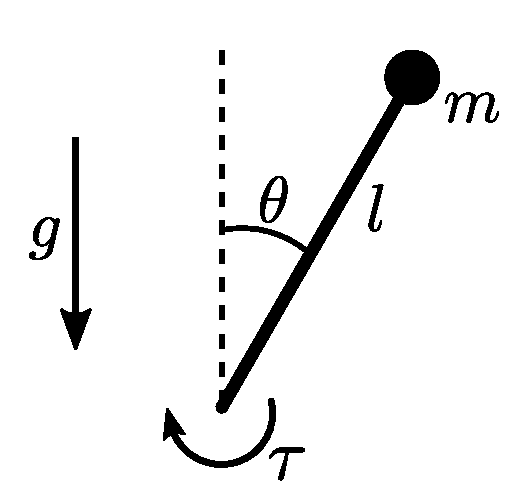
\includegraphics[width=.3\textwidth]{figures/system}
  \end{figure}
  %
  \small
  \begin{flalign}
    \hspace{1.5cm}
    a&=\frac{g}{l} \ \ , \ \ \ b = \frac{k}{m} \ \ , \ \ \ c =  \frac{1}{m l^2}  \ \ , \ \ \ u = \tau   \ \ , \ \ \ \text{s.t.}, & \nonumber
  \end{flalign}
  \normalsize
  \begin{flalign}
    \hspace{1.5cm}
    \dot{x_1} &= x_2 & \nonumber \\
    \dot{x_2} &= a \sin x_1 - b x_2 + c u & \nonumber
  \end{flalign}
\end{frame}

\begin{frame}{Introduction}{The System}
  \begin{figure}[H]
    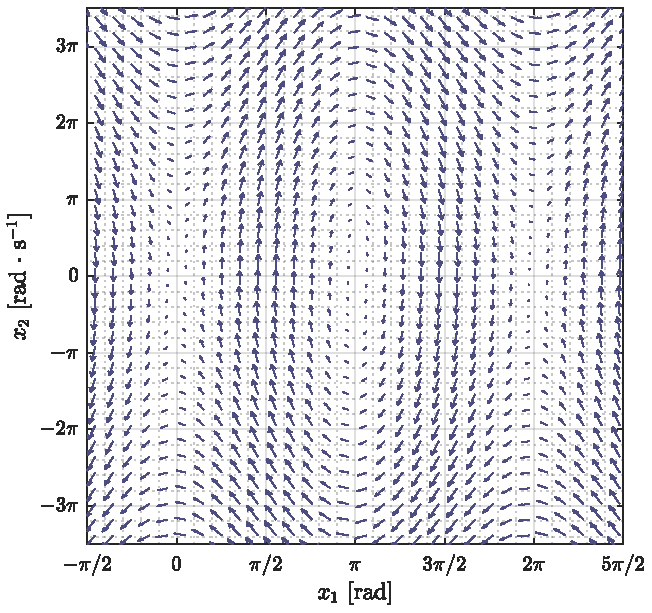
\includegraphics[width=.85\textwidth]{figures/modelPhasePlot}
  \end{figure}
\end{frame}

\begin{frame}{Introduction}{Linear Control}
  \begin{figure}[H]
    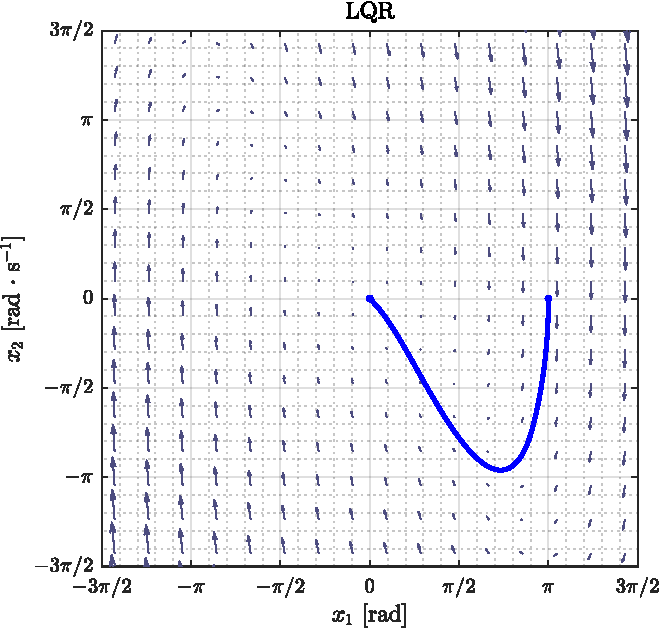
\includegraphics[width=.55\textwidth]{figures/LQRphasePlot}
  \end{figure}
\end{frame}


%-------Feedback Linearization--------------------------------------------------

\begin{frame}{Nonlinear Control Design}{Feedback Linearization}
  \begin{flalign}
    \dot{x_1} &= x_2  & \nonumber \\
    \dot{x_2} &= \hat{h}_1(x) + \hat{h}_2(x)  + \hat{g}(x) u \nonumber
  \end{flalign}
  \begin{flalign}
    u &= \frac{1}{\hat{g}(x)} (-\hat{h}_1(x) + v ) & \nonumber
  \end{flalign}
  \begin{flalign}
    \dot{x_1} &= x_2  &  \nonumber \\
    \dot{x_2} &= \hat{h}_2(x) + v  & \nonumber
  \end{flalign}
  \begin{figure}[H]
    \vspace{-5cm}
    \begin{minipage}{0.45\linewidth}    
    \end{minipage}\hfill      
    \begin{minipage}{0.45\linewidth}
      \begin{figure}[H]
        \centering
        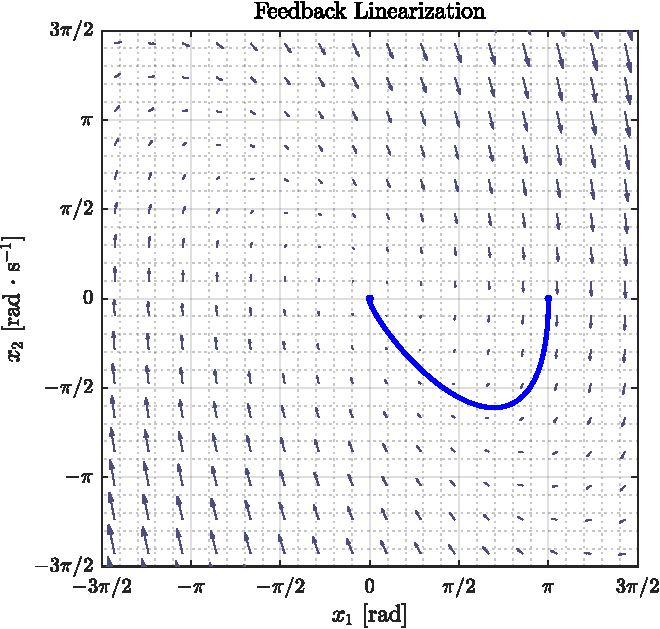
\includegraphics[width=1\linewidth]{figures/feedbackLinearizationPhasePlot}
      \end{figure}                
    \end{minipage}\hfill \\
  \end{figure}
\end{frame}


%-------Sliding Mode----------------------------------------------------------


\begin{frame}{Nonlinear Control Design}{Sliding Mode}
\vspace{-15pt}
\begin{flalign}
  s &= a_1 x_1 + x_2 = 0 \ \ \ \ \ \ \ \ \ \ V = \frac{1}{2} s^2   & \nonumber 
\end{flalign}
\begin{flalign}
  \dot{V} &\leq g(x) |s| \left|\frac{a_1 x_2 + h(x)}{g(x)}\right| + g(x) s u  & \nonumber
\end{flalign}
\begin{flalign}
\dot{V} &\leq g(x) |s| \left|\frac{a_1 x_2 + h(x)}{g(x)}\right| -  g(x) \text{sgn}(s) s \left|\frac{a_1 x_2 + h(x)}{g(x)}\right| & \nonumber
\end{flalign}
\begin{flalign}
u &= - \text{sgn}(s) \varrho(x) \ \ \ \ \ \text{where,}\ \ \ \varrho (x) \geq \left| \frac{a_1 x_2 + h(x)}{g(x)} \right| \ \ \ & \nonumber
\end{flalign}
\begin{flalign}
u &= - \text{sgn}(s) \beta(x) \ \ \ \ \ \text{where,}\ \ \ \beta(x) = \varrho(x) + \beta_0  \ \ \ \ \ \text{and}\ \ \  \beta_0 > 0 \ \ \ & \nonumber
\end{flalign}
\end{frame}

\begin{frame}{Nonlinear Control Design}{Sliding Mode}
\begin{figure}[H]
  \begin{minipage}{0.45\linewidth}
    \begin{figure}[H]
      \centering
      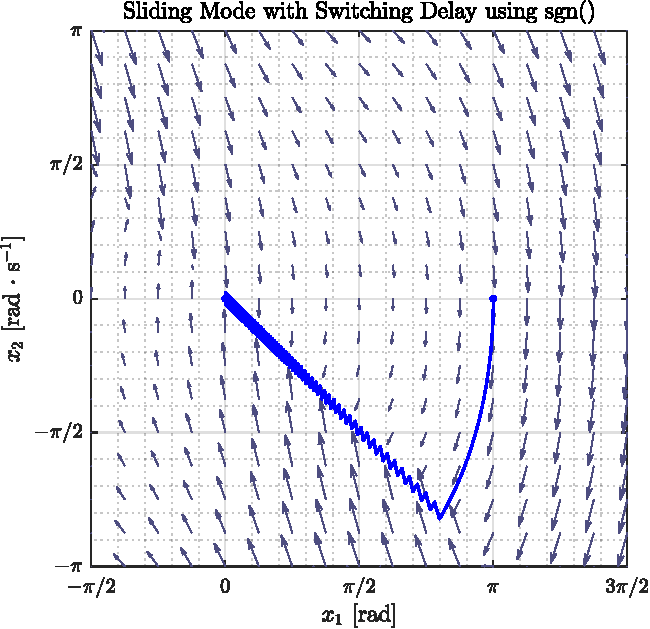
\includegraphics[width=\linewidth]{figures/slidingModeSgn}
    \end{figure}        
  \end{minipage}\hfill      
  \begin{minipage}{0.45\linewidth}
    \begin{figure}[H]
      \centering
      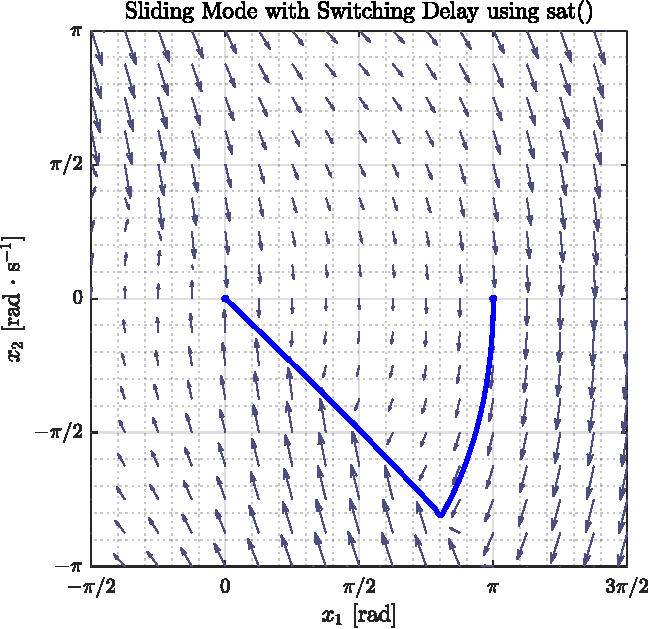
\includegraphics[width=1\linewidth]{figures/slidingModeSat}
    \end{figure}                
  \end{minipage}\hfill \\
\end{figure}
\end{frame}

\begin{frame}{Nonlinear Control Design}{Sliding Mode}
\vspace{-15pt}
\begin{flalign}
\dot{s} &= a_1 x_2 + h(x) + g(x) u \ \ \ , \ \ \ \ \text{where}\ \ \ u = -\frac{a_1 x_2 + \hat{h}(x)}{\hat{g}(x)} + v &  \nonumber
\end{flalign}
\begin{flalign}
\dot{s} &= \delta(x) + g(x) v    \ \ \ , \ \ \ \ \text{where}\ \ \   \delta(x) = a_1 (1- \frac{g(x)}{\hat{g}(x)}) x_2 + h(x) - \frac{g(x)}{\hat{g}(x)} \hat{h}(x)  &  \nonumber
\end{flalign}
%
\begin{flalign}
v &= -\beta(x) \text{sgn}(s)  \ \ \ , \ \ \ \ \text{where}\ \ \  \beta(x) \geq \varrho(x) +\beta_0   \ \ \ , \ \ \ \text{and}\ \ \ \varrho(x) \geq \left| \frac{\delta(x)}{\hat{g}(x)} \right|   & \nonumber
\label{eq:slidingControlLawSplit}
\end{flalign}
\end{frame}

\begin{frame}{Nonlinear Control Design}{Sliding Mode}
\begin{figure}[H]
  \begin{minipage}{0.45\linewidth}
    \begin{figure}[H]
      \centering
      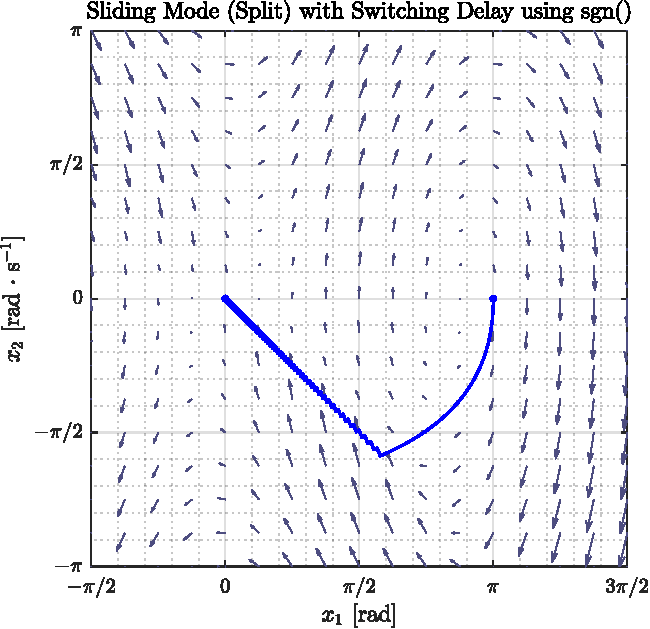
\includegraphics[width=\linewidth]{figures/slidingModeSplitSgn}
    \end{figure}        
  \end{minipage}\hfill      
  \begin{minipage}{0.45\linewidth}
    \begin{figure}[H]
      \centering
      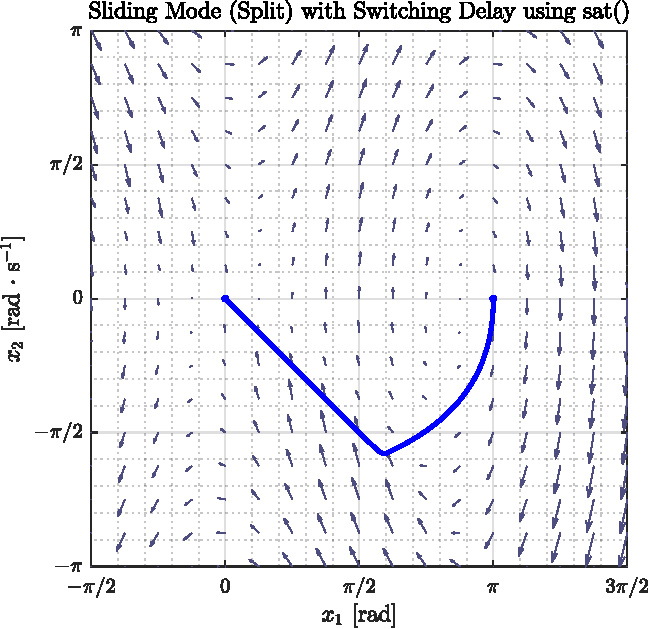
\includegraphics[width=1\linewidth]{figures/slidingModeSplitSat}
    \end{figure}                
  \end{minipage}\hfill \\
\end{figure}
\end{frame}

%-------Lyapunov Redesign------------------------------------------------------

\begin{frame}{Nonlinear Control Design}{Lyapunov Redesign}
\small
\begin{flalign}
  %\hspace{-15pt}
  \delta &= \frac{1}{\hat{g}(x)} \left[(h(x) - \hat{h}(x)) + (g(x)  - \hat{g}(x)) u\right] \ \ \ \ \text{where,} \ \ \ \ \ u = \psi(x) + v_1 & \nonumber
\end{flalign}
%\begin{flalign}
%\hspace{-15pt}
%\delta &= \frac{1}{\hat{g}(x)}
%\left[
%\frac{h_1(x)\hat{g}(x) -g(x)\hat{h}_1(x) }{\hat{g}(x)} + h_2(x) - \hat{h}_2(x)
%+\frac{g(x)-\hat{g}(x)}{\hat{g}(x)} v
%\right]
%+ \frac{g(x)-\hat{g}(x)}{\hat{g}(x)} v_1 & \nonumber
%\end{flalign}
\begin{flalign}
  \delta &= \frac{1}{\hat{c}}\left(   \frac{a \hat{c} - \hat{a} c}{\hat{c}} \sin x_1 + (\hat{b}-b) x_2 + \frac{c-\hat{c}}{\hat{c}} (k_1 x_1 + k_2 x_2)    \right) +\frac{c-\hat{c}}{\hat{c}} v_1   & \nonumber
\end{flalign}

\begin{flalign}
  |\delta| &\leq \rho \rVert \vec{x} \rVert_2 + \kappa_0 \left| v_1 \right| \ \ \ \ \text{where,}  & \nonumber
\end{flalign}
\begin{flalign}
  \rho =&  \frac{1}{\hat{c}}   \left(  \left| \frac{a \hat{c} - \hat{a} c}{\hat{c}} \right| + \left| \hat{b}-b \right| + \left| \frac{c-\hat{c}}{\hat{c}} \right| \sqrt{k_1^2 + k_2^2}  \right)     \ \text{ and } \ \kappa_0 = \left| \frac{c-\hat{c}}{\hat{c}} \right|  & \nonumber
\end{flalign}
\normalsize
\end{frame}

\begin{frame}{Nonlinear Control Design}{Lyapunov Redesign}
\begin{flalign}
  v_1 &= -\eta (t,x) \text{sgn}(\omega) & \nonumber
\end{flalign}
\begin{flalign}
  \omega &= \frac{\partial V}{\partial \vec{x}} G(\vec{x}) \ \ \ \ \text{where,}\ \ \ \ G(x) = [\ 0 \ \ \hat{g}(x) \ ]^{\text{T}} & \nonumber
\end{flalign}
\begin{flalign}
  \eta(t,x) &\geq \rho(t,x)/(1 - \kappa_0) & \nonumber
\end{flalign}
\begin{flalign}
v_1 &=
  \begin{cases}
    \ \ -\eta(t,x)   \omega / \rVert \omega \rVert_2, & \ \text{if} \ \ \eta(t,x) \rVert \omega \rVert_2 \geq \varepsilon \\
    \ \ -\eta^2(t,x) \omega / \varepsilon,            & \ \text{if} \ \ \eta(t,x) \rVert \omega \rVert_2 < \varepsilon \ \ , \ \ \ \ \eta(t,x) \geq \rho(t,x) / (1-\kappa_0) 
  \end{cases} &  \nonumber
\end{flalign}
\end{frame}

\begin{frame}{Nonlinear Control Design}{Lyapunov Redesign}
  \begin{figure}[H]
    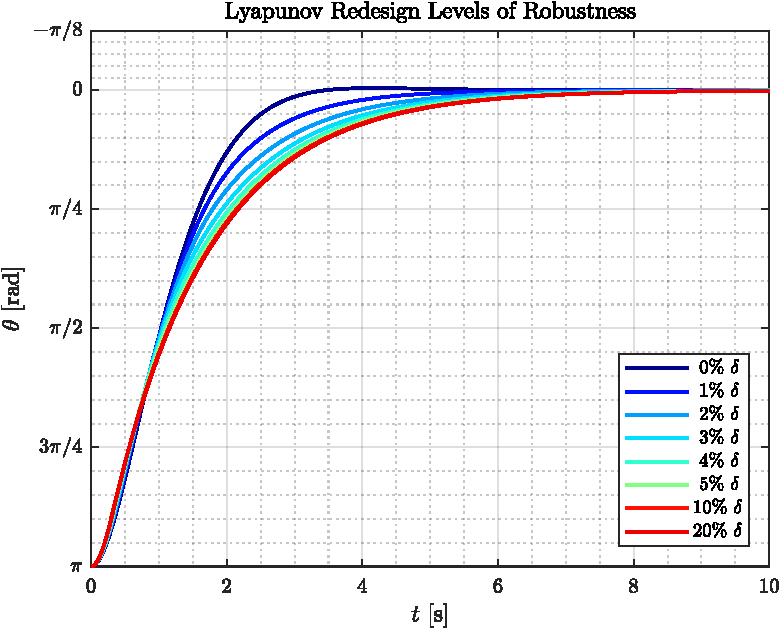
\includegraphics[width=.55\textwidth]{figures/lyapunovRedesignRobustness}
  \end{figure}
\end{frame}

\begin{frame}{Nonlinear Control Design}{Lyapunov Redesign}
  \begin{figure}[H]
    \begin{minipage}{0.45\linewidth}
      \begin{figure}[H]
        \centering
        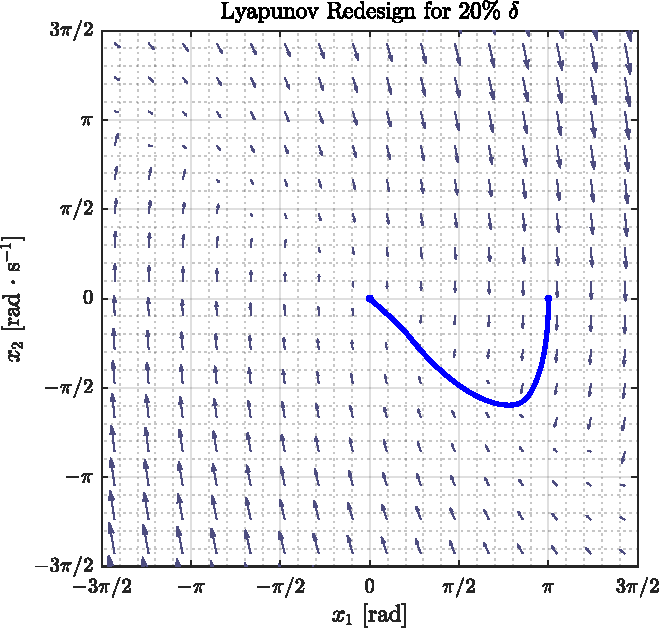
\includegraphics[width=\linewidth]{figures/lyapunovRedesignPhasePlot}
      \end{figure}        
    \end{minipage}\hfill      
    \begin{minipage}{0.45\linewidth}
      \begin{figure}[H]
        \centering
        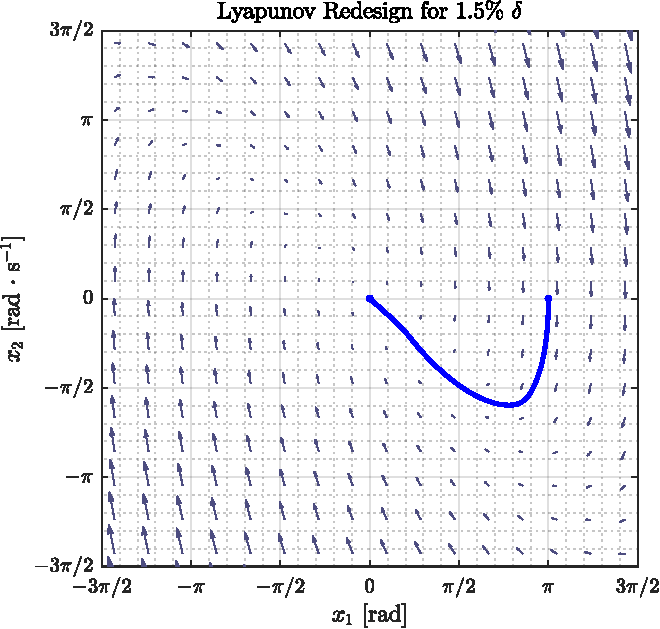
\includegraphics[width=1\linewidth]{figures/lyapunovRedesignPhasePlot2}
      \end{figure}                
    \end{minipage}\hfill \\
  \end{figure}
\end{frame}


%-------Robustness to Parameter Variation--------------------------------------

\begin{frame}{Results}{Robustness to Parameter Variation}
\begin{figure}[H]
  \begin{minipage}{0.45\linewidth}
    \begin{figure}[H]
      \centering
      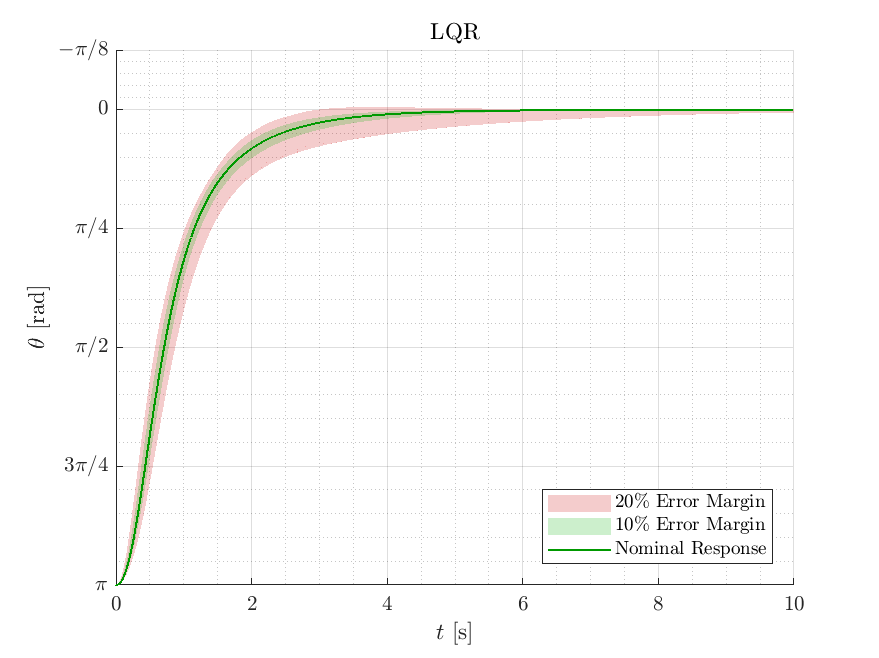
\includegraphics[width=\linewidth]{figures/LQR}
    \end{figure}        
  \end{minipage}\hfill      
  \begin{minipage}{0.45\linewidth}
    \begin{figure}[H]
      \centering
      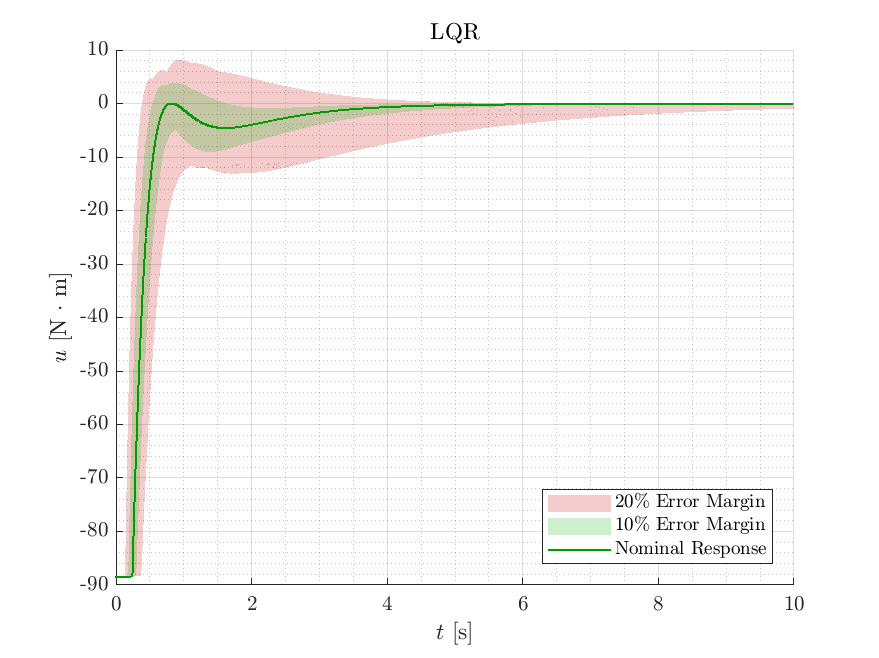
\includegraphics[width=1\linewidth]{figures/LQR_u}
    \end{figure}                
  \end{minipage}\hfill \\
\end{figure}
\end{frame}

\begin{frame}{Results}{Robustness to Parameter Variation}
\begin{figure}[H]
  \begin{minipage}{0.45\linewidth}
    \begin{figure}[H]
      \centering
      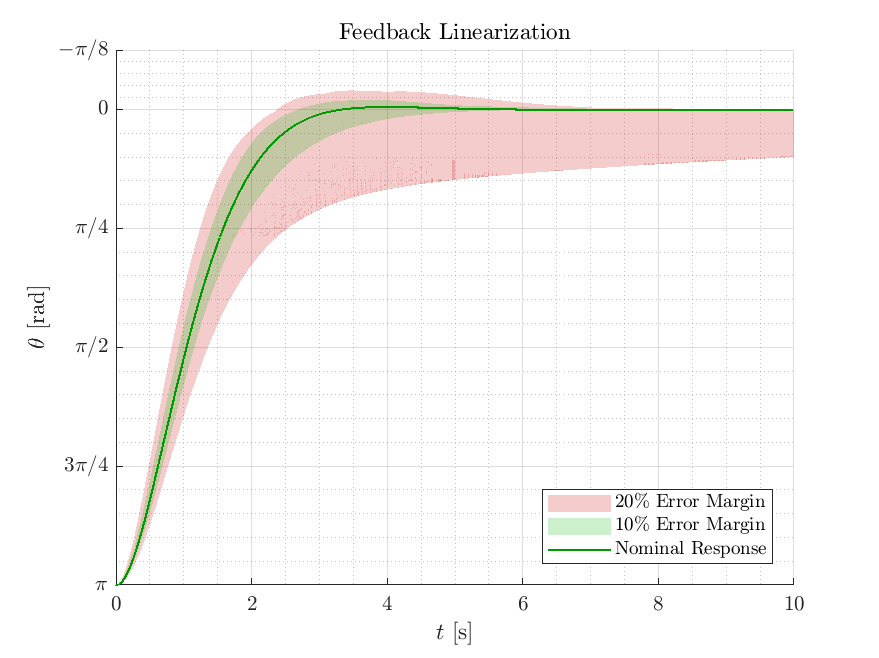
\includegraphics[width=\linewidth]{figures/feedbackLinearization}
    \end{figure}        
  \end{minipage}\hfill      
  \begin{minipage}{0.45\linewidth}
    \begin{figure}[H]
      \centering
      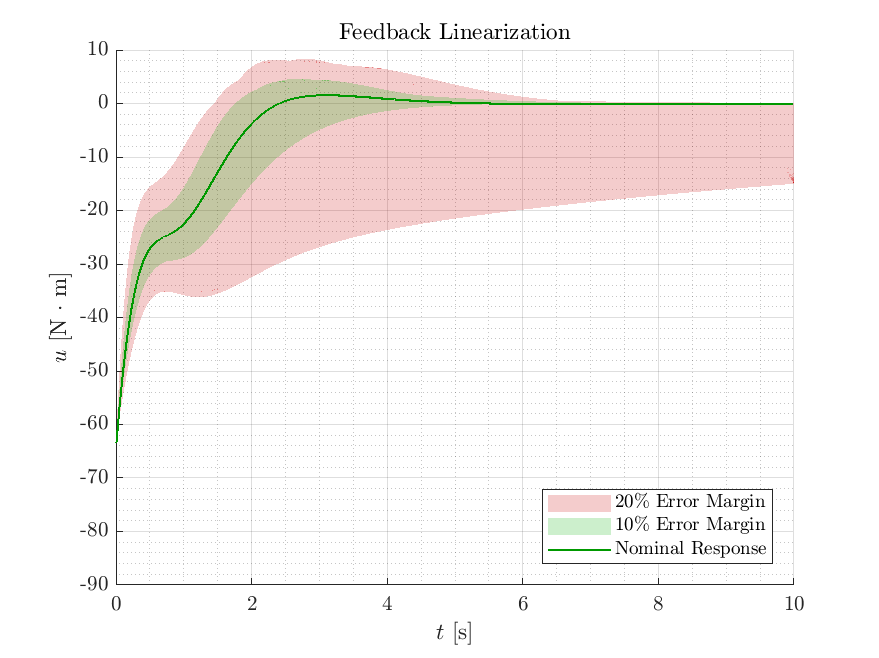
\includegraphics[width=1\linewidth]{figures/feedbackLinearization_u}
    \end{figure}                
  \end{minipage}\hfill \\
\end{figure}
\end{frame}

\begin{frame}{Results}{Robustness to Parameter Variation}
\begin{figure}[H]
  \begin{minipage}{0.45\linewidth}
    \begin{figure}[H]
      \centering
      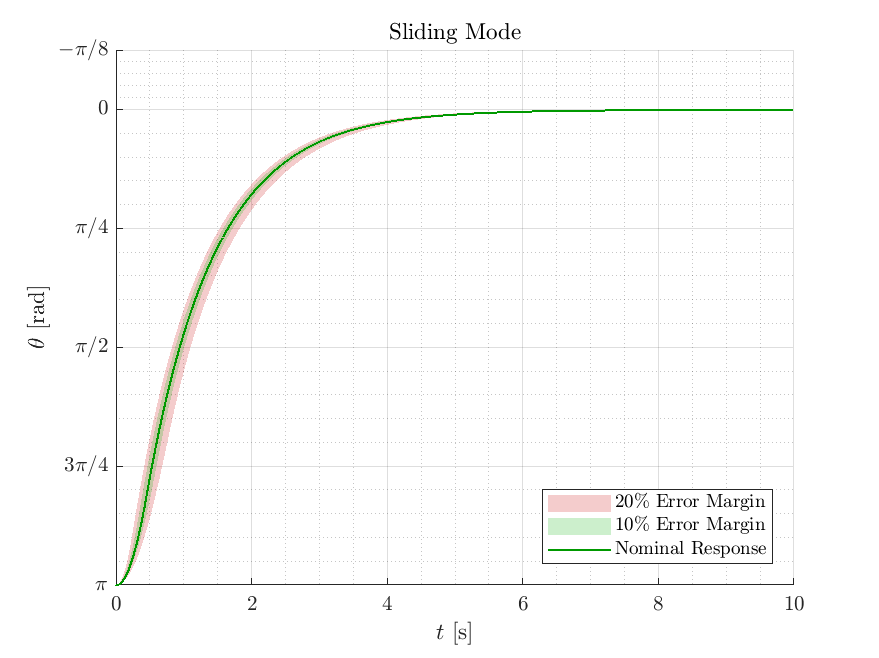
\includegraphics[width=\linewidth]{figures/slidingMode}
    \end{figure}        
  \end{minipage}\hfill      
  \begin{minipage}{0.45\linewidth}
    \begin{figure}[H]
      \centering
      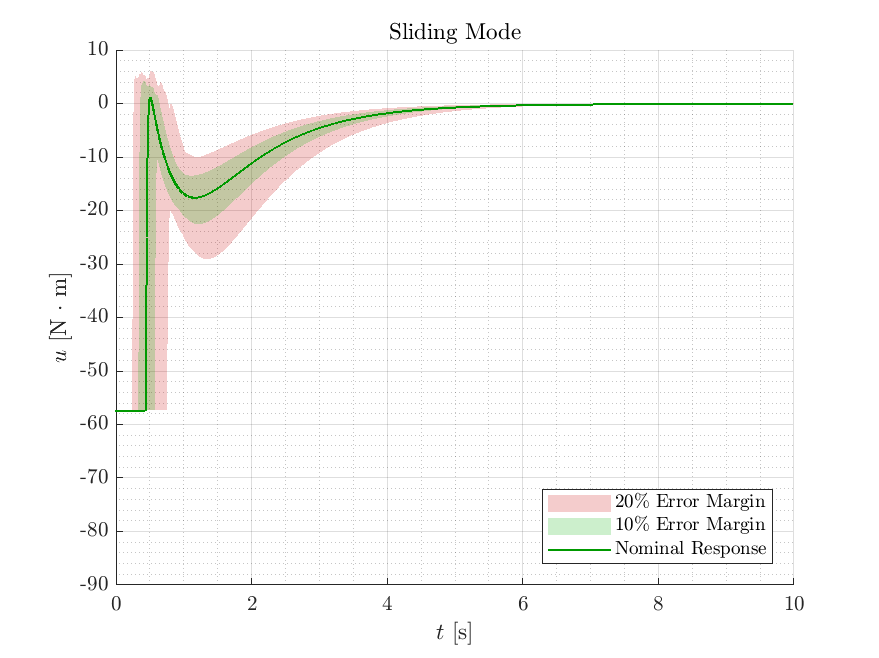
\includegraphics[width=1\linewidth]{figures/slidingMode_u}
    \end{figure}                
  \end{minipage}\hfill \\
\end{figure}
\end{frame}

\begin{frame}{Results}{Robustness to Parameter Variation}
\begin{figure}[H]
  \begin{minipage}{0.45\linewidth}
    \begin{figure}[H]
      \centering
      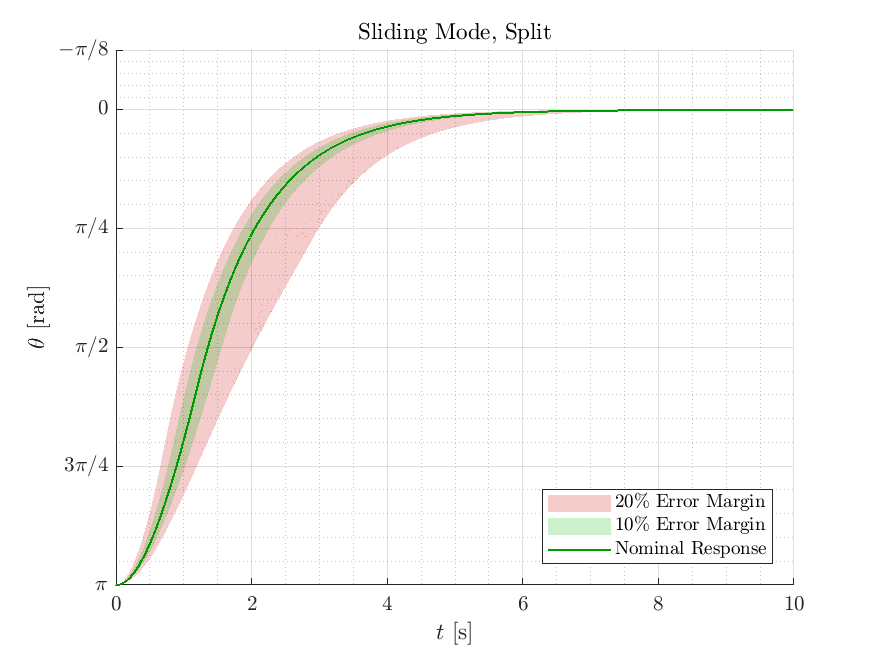
\includegraphics[width=\linewidth]{figures/slidingModeSplit}
    \end{figure}        
  \end{minipage}\hfill      
  \begin{minipage}{0.45\linewidth}
    \begin{figure}[H]
      \centering
      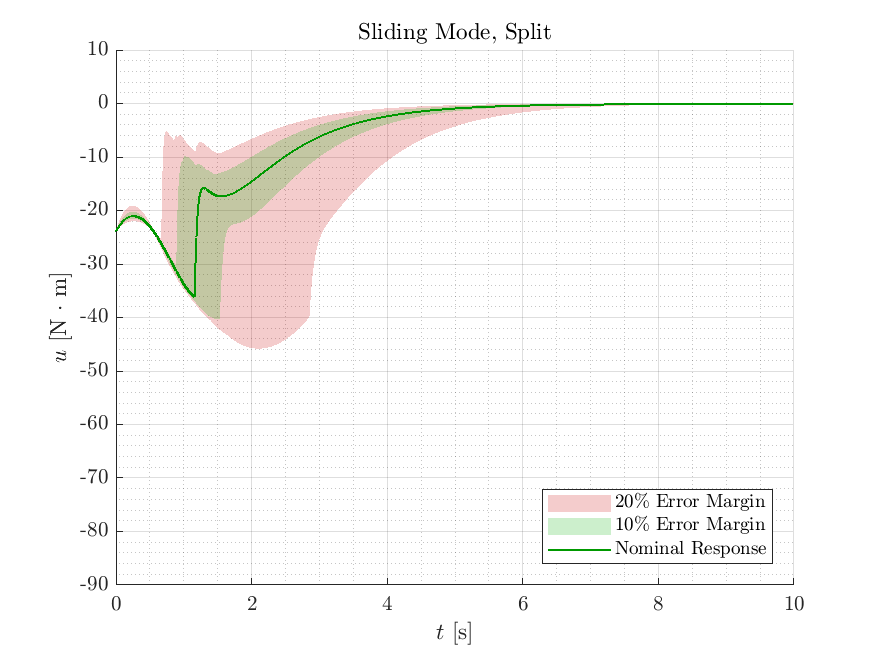
\includegraphics[width=1\linewidth]{figures/slidingModeSplit_u}
    \end{figure}                
  \end{minipage}\hfill \\
\end{figure}
\end{frame}

\begin{frame}{Results}{Robustness to Parameter Variation}
\begin{figure}[H]
  \begin{minipage}{0.45\linewidth}
    \begin{figure}[H]
      \centering
      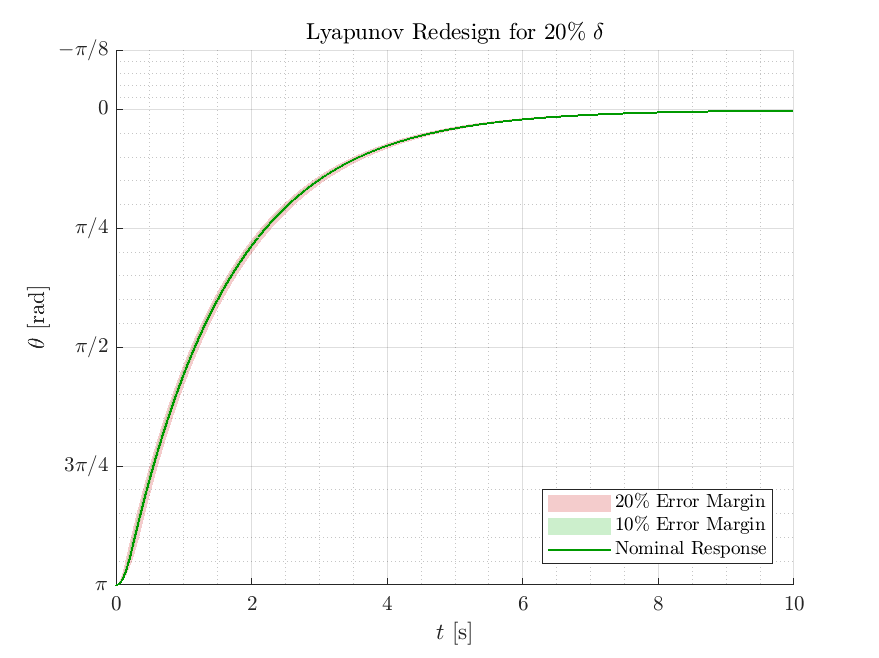
\includegraphics[width=\linewidth]{figures/lyapunovRedesign}
    \end{figure}        
  \end{minipage}\hfill      
  \begin{minipage}{0.45\linewidth}
    \begin{figure}[H]
      \centering
      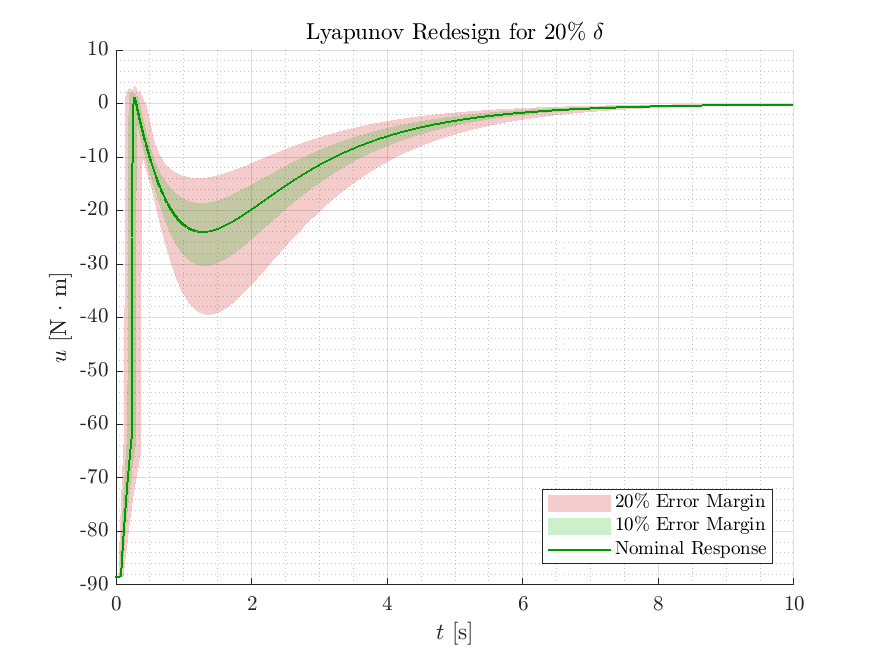
\includegraphics[width=1\linewidth]{figures/lyapunovRedesign_u}
    \end{figure}                
  \end{minipage}\hfill \\
\end{figure}
\end{frame}

\begin{frame}{Results}{Robustness to Parameter Variation}
\begin{figure}[H]
  \begin{minipage}{0.45\linewidth}
    \begin{figure}[H]
      \centering
      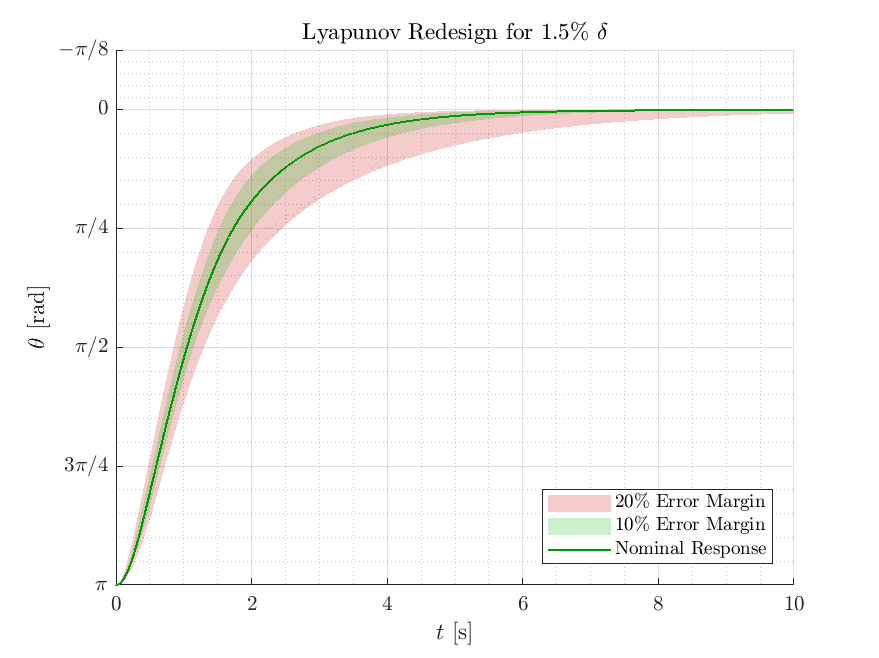
\includegraphics[width=\linewidth]{figures/lyapunovRedesign2}
    \end{figure}        
  \end{minipage}\hfill      
  \begin{minipage}{0.45\linewidth}
    \begin{figure}[H]
      \centering
      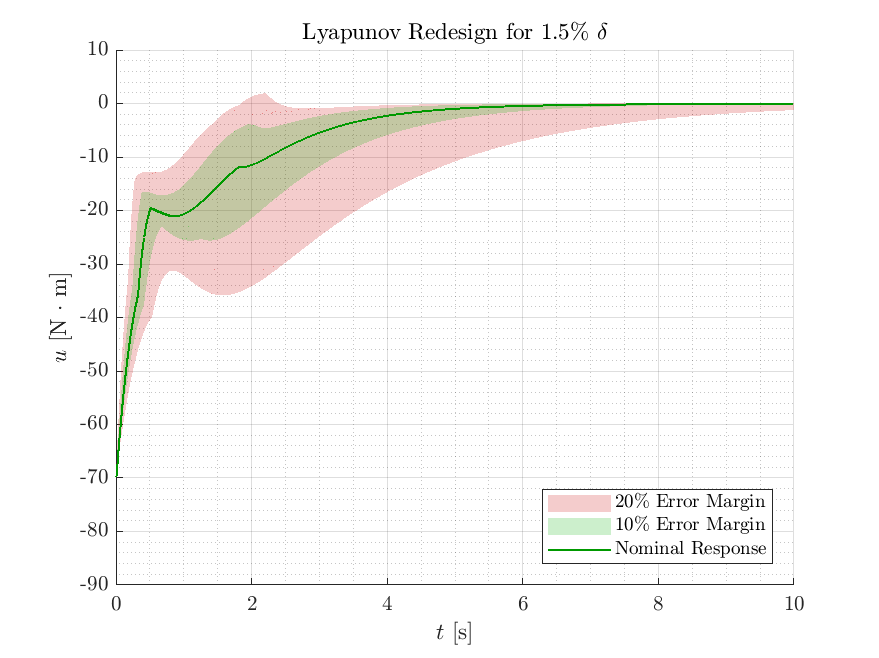
\includegraphics[width=1\linewidth]{figures/lyapunovRedesign2_u}
    \end{figure}                
  \end{minipage}\hfill \\
\end{figure}
\end{frame}


%-------Robustness to Input Noise-----------------------------------------------

\begin{frame}{Results}{Robustness to Input Noise}
\begin{figure}[H]
  \begin{minipage}{0.45\linewidth}
    \begin{figure}[H]
      \centering
      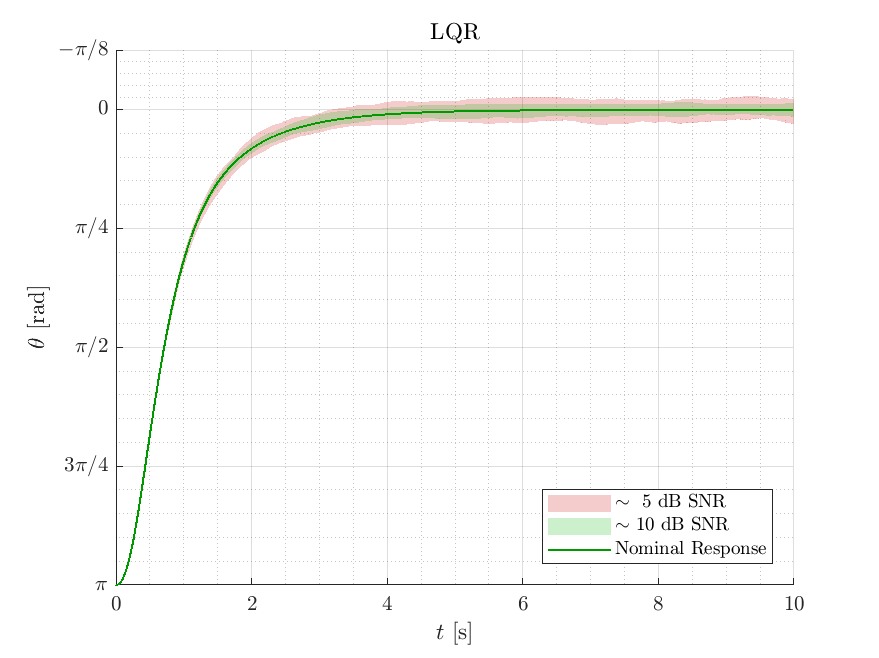
\includegraphics[width=\linewidth]{figures/LQRinputNoise}
    \end{figure}        
  \end{minipage}\hfill      
  \begin{minipage}{0.45\linewidth}
    \begin{figure}[H]
      \centering
      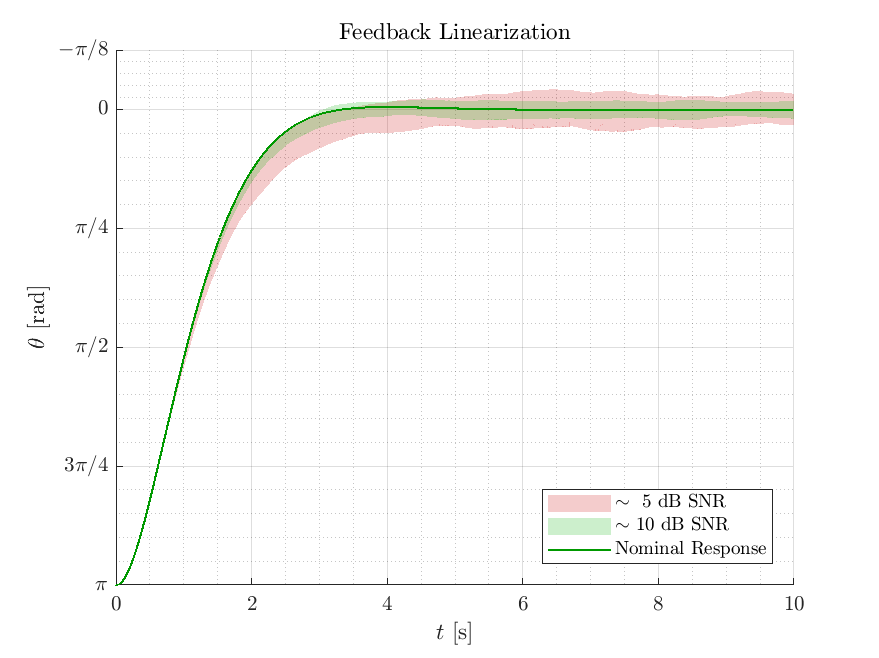
\includegraphics[width=1\linewidth]{figures/feedbackLinearizationInputNoise}
    \end{figure}                
  \end{minipage}\hfill \\
\end{figure}
\end{frame}

\begin{frame}{Results}{Robustness to Input Noise}
\begin{figure}[H]
\begin{minipage}{0.45\linewidth}
  \begin{figure}[H]
    \centering
    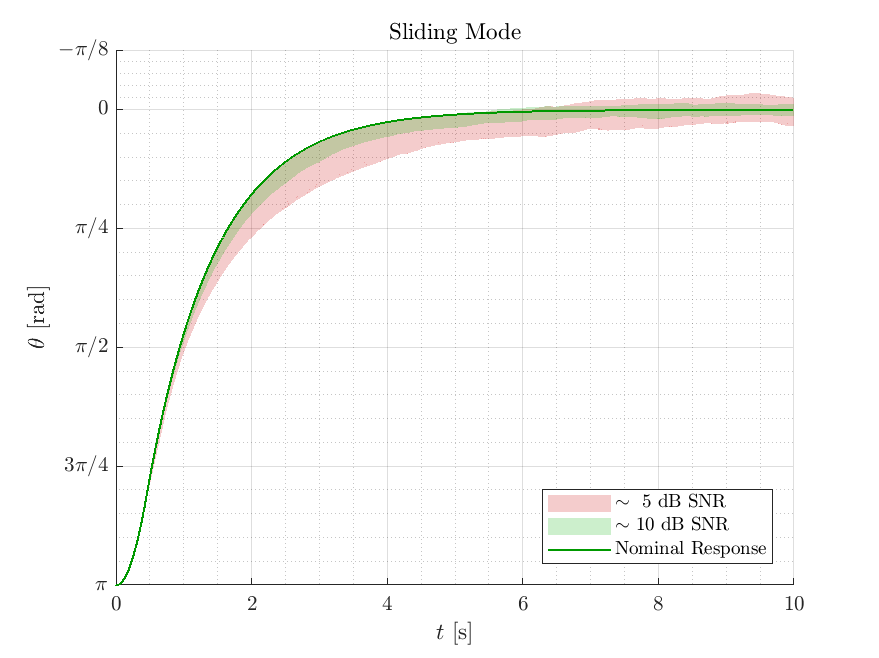
\includegraphics[width=\linewidth]{figures/slidingModeInputNoise}
  \end{figure}        
\end{minipage}\hfill      
\begin{minipage}{0.45\linewidth}
  \begin{figure}[H]
    \centering
    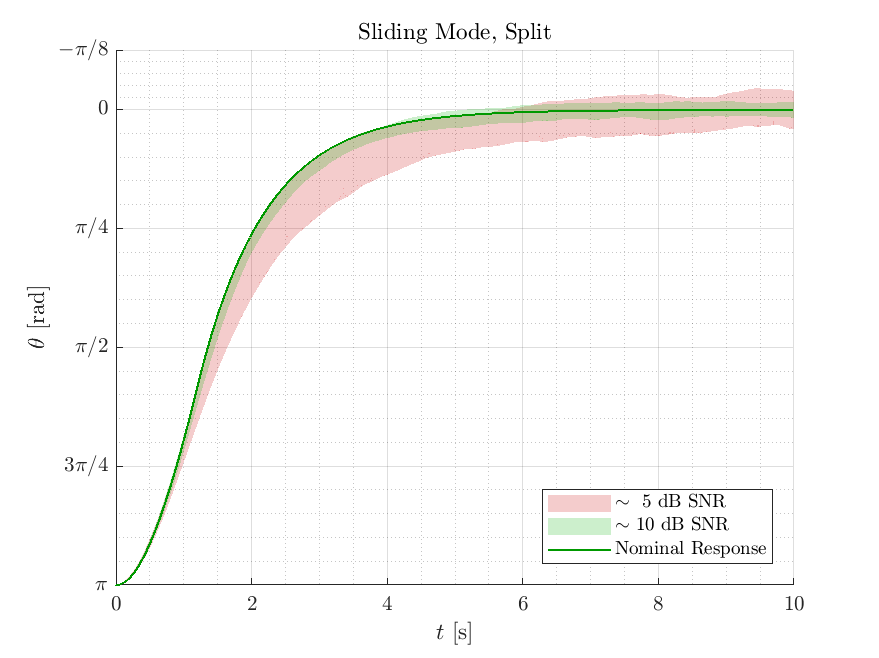
\includegraphics[width=1\linewidth]{figures/slidingModeSplitInputNoise}
  \end{figure}                
\end{minipage}\hfill \\
\end{figure}
\end{frame}

\begin{frame}{Results}{Robustness to Input Noise}
\begin{figure}[H]
  \begin{minipage}{0.45\linewidth}
    \begin{figure}[H]
      \centering
      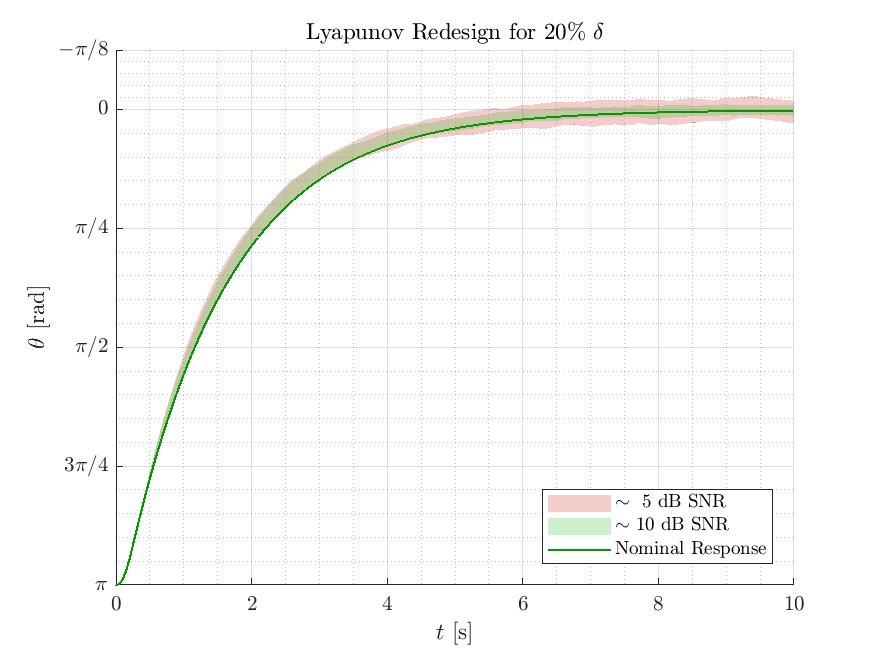
\includegraphics[width=\linewidth]{figures/lyapunovRedesignInputNoise}
    \end{figure}        
  \end{minipage}\hfill      
  \begin{minipage}{0.45\linewidth}
    \begin{figure}[H]
      \centering
      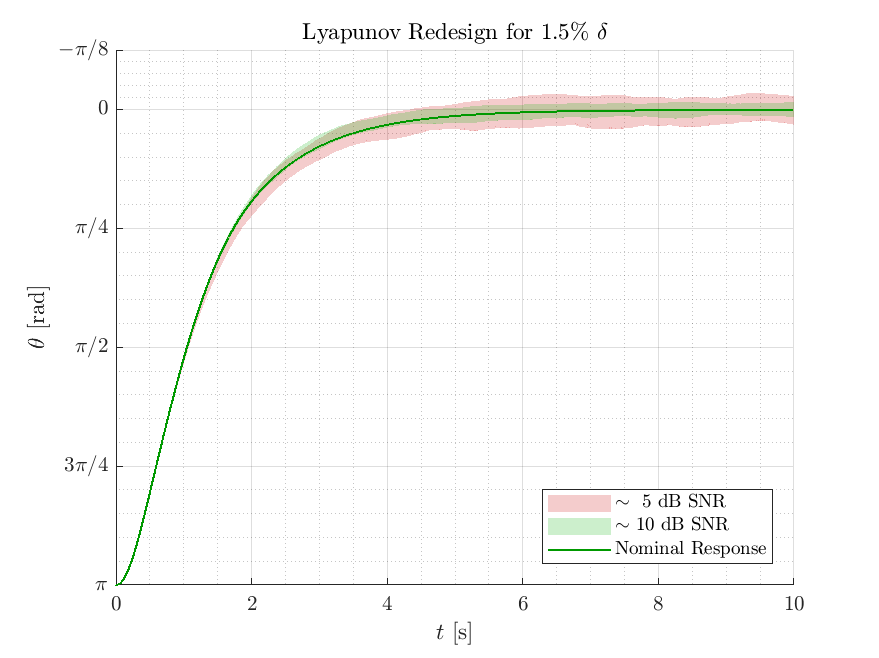
\includegraphics[width=1\linewidth]{figures/lyapunovRedesign2InputNoise}
    \end{figure}                
  \end{minipage}\hfill \\
\end{figure}
\end{frame}
